% LaTeX source for joint paper on SUNDIALS
% Version of 18 August 2003

\documentclass[acmtoms]{acmtrans2m}
\usepackage{amsmath, amssymb}
\usepackage{epsfig}
\usepackage{tabularx}
%\usepackage{showlabels}

\newcommand{\dfdy}{\frac{\partial f}{\partial y}}
\newcommand{\dfdyI}{\partial f / \partial y}
\newcommand{\dfdpi}{\frac{\partial f}{\partial p_i}}
\newcommand{\dfdpiI}{\partial f / \partial p_i}

\newcommand{\mb}[1]{{\mbox{\scriptsize #1}}}

\makeatletter
\newcommand{\figcaption}{\def\@captype{figure}\caption}
\newcommand{\tabcaption}{\def\@captype{table}\caption}
\makeatother

\acmVolume{V}
\acmNumber{N}
\acmYear{Y}
\acmMonth{Month}

\markboth{R. Serban and A.C. Hindmarsh}
{CVODES: An ODE solver with sensitivity analysis capabilities}

\title{CVODES: An ODE solver with sensitivity analysis capabilities}

\author{RADU SERBAN and ALAN C. HINDMARSH \\
  Center for Applied Scientific Computing \\
  Lawrence Livermore National Laboratory}

\begin{abstract}
CVODES, which is part of the SUNDIALS software suite,
is a stiff and nonstiff ordinary differential equation initial 
value problem solver with sensitivity analysis capabilities. 
CVODES is written in a data-independent manner, with a highly 
modular structure to allow incorporation of different 
preconditioning and/or linear solver methods. It shares with the 
other SUNDIALS solvers several common modules, most notably the 
generic kernel of vector operations and a set of generic linear 
solvers and preconditioners.

CVODES solves the IVP by one of two methods -- backward differentiation 
formula or Adams-Moulton -- both implemented in a variable-step, 
variable-order form. The forward sensitivity module in CVODES implements 
the simultaneous corrector method, as well as two flavors of 
staggered corrector methods. Its adjoint sensitivity module 
provides a combination of checkpointing and cubic Hermite interpolation 
for the efficient generation of the forward solution during the adjoint 
system integration.

We describe the current capabilities of CVODES, its design principles,
and its user interface.  We also give an example problem to illustrate
the performance of CVODES.

\end{abstract}

\category{G.4}{Mathematical Software}{Algorithm design and analysis}

\category{G.1.7}{Numerical Analysis}{Ordinary Differential Equations}
[Initial value problems \and Multistep methods \and Stiff equations]

%\category{G.1.m}{Miscellaneous}{Sensitivity Analysis}
%[Forward methods \and Adjoint methods]

\terms{Algorithms, Design}

\keywords{ODEs, Forward Sensitivity Analysis, Adjoint Sensitivity Analysis}

%=======================================================================

\begin{document}

\setcounter{page}{1}

\begin{bottomstuff}
Authors' address: 
Radu Serban, 
Lawrence Livermore National Laboratory, P.O. Box 808, L-560,
Livermore, CA 94551; email: {\tt radu@llnl.gov};
Alan C. Hindmarsh,
Lawrence Livermore National Laboratory, P.O. Box 808, L-560,
Livermore, CA 94551; email: {\tt alanh@llnl.gov};
\newline
This work was performed under the auspices of the
U.S. Department of Energy by the University of California,
Lawrence Livermore National Laboratory, under contract No.
W-7405-Eng-48.
\end{bottomstuff}

\maketitle

%=======================================================================
% Include sections

\section{Introduction}\label{s:introduction}

Fortran solvers for ODE initial value problems (IVPs) are widespread and heavily used. 
Two solvers that have been written at LLNL in the past are VODE \cite{BBH:89} 
and VODPK \cite{Byr:92}.
%
%% VODE is a general purpose solver that includes methods for stiff
%% and nonstiff systems, and in the stiff case uses direct methods (full or
%% banded) for the solution of the linear systems that arise at each implicit
%% step. Externally, VODE is very similar to the well known solver
%% LSODE \cite{RaHi:94}. 
%% VODPK is a variant of VODE that uses a preconditioned Krylov 
%% (iterative) method for the solution of the linear systems. VODPK is a powerful 
%% tool for large stiff systems because it combines established methods for stiff 
%% integration, nonlinear iteration, and Krylov (linear) iteration with a problem-specific
%% treatment of the dominant source of stiffness, in the form of the user-supplied
%% preconditioner matrix~\cite{BrHi:89}.
%
The capabilities of both VODE and VODPK have been combined in the C-language 
packages CVODE~\cite{CoHi:96} and PVODE~\cite{ByHi:99}, later merged under the
suite SUNDIALS~\cite{HBGLSSW:04} into one solver, CVODE, which runs on both
serial and parallel computers. Besides CVODE, the other two basic solvers in SUNDIALS
are IDA, a solver for differential-algebraic equation (DAE) systems, and
KINSOL, a Newton-Krylov (GMRES) solver for nonlinear algebraic systems.

In recent years, research and development related to the SUNDIALS solvers has
focused on sensitivity analysis to address questions related to unknown 
parameters in the mathematical models under consideration.
Essentially, sensitivity analysis quantifies the relationship between
changes in model parameters and changes in model outputs. Such information 
is crucial for design optimization, parameter estimation, optimal control, data
assimilation, process sensitivity, and experimental design.
%%
%% There are two main approaches to sensitivity analysis.
%% {\em Forward sensitivity analysis} has been proven to be very efficient for
%% problems in which the sensitivities of a (potentially) very large
%% number of quantities with respect to relatively few parameters are
%% needed.  However, for problems where the number of uncertain
%% parameters is large, the forward sensitivity method becomes
%% computationally intractable.  The {\em adjoint sensitivity method}, also called
%% reverse method, is advantageous in the complementary situation where the sensitivities of
%% a few quantities with respect to a large number of parameters are needed.
%%
SUNDIALS is currently being expanded to include sensitivity-capable variants of all
its basic solvers. The first one, CVODES, released in July 2002, 
is written with a functionality and user interface that is a superset of that of CVODE. 
In that sense, CVODES is backward compatible with CVODE.
Sensitivity analysis capabilities, both forward and adjoint, have been added to 
the main integrator. Enabling forward sensititivity computations 
in CVODES will result in the code integrating the so-called 
{\em sensitivity equations} simultaneously with the original IVP, 
yielding both the solution and its sensitivity with respect to parameters in the model. 
Adjoint sensitivity analysis involves integration of the 
original IVP forward in time followed by the integration of the so-called 
{\em adjoint equations} backwards in time. 
CVODES provides the infrastructure needed to integrate any final-condition ODE
dependent on the solution of the original IVP (not only the adjoint system). 

Development of CVODES was concurrent with a redesign of the vector operations module 
(NVECTOR) across the SUNDIALS suite. The key feature of the new NVECTOR module is that it
is written in terms of abstract vector operations with the actual vector kernels attached
by a particular implementation (such as serial or parallel). This allows
writing the SUNDIALS solvers in a manner independent of the actual NVECTOR vector
implementation (which can be user-supplied), as well as allowing more than one 
NVECTOR module linked into an executable file. This feature is essential in certain
sensitivity analysis computations and impossible in Fortran.

Like all the SUNDIALS solvers, CVODES is written in ANSI-C.
Among the advantages of using C, we mention portability of the solver libraries, 
compiler availability, a standard dynamic memory allocation mechanism, and the
ability to define complex data structures.
The design of the SUNDIALS solvers does not impede interlanguage operability. 
As an example of using a SUNDIALS solver with Fortran user code, the reader is 
refered to the Fortran-C interface provided for CVODE \cite{HiSe:04cvode,HBGLSSW:04}.

The rest of this paper is organized as follows. In Section~\ref{s:algorithms}, the
algorithms implemented in CVODES for ODE integration and forward and adjoint 
sensitivity analysis are presented. The CVODES code organization and relationship
to SUNDIALS is discussed in Section~\ref{s:organization}, while Section~\ref{s:usage}
gives a high-level overview of the solver usage and general
philosophy of the user interface. 
Section~\ref{s:parallel} presents an example problem and its solution on a
parallel machine.
We conclude with indications on software availability
in Section~\ref{s:availability} and with some final remarks and directions
of current and future development in Section~\ref{s:conclusions}.

\section{Algorithms}\label{s:algorithms}

CVODES solves initial value problems with free parameters. 
Such problems can be stated as
\begin{equation}\label{e:ivp}
\dot{y}  = f(t,\,y,\,p) \, , \quad y(t_0)  = y_0(p) \, ,
\end{equation}
where $y \in {\bf R}^N$ is  the vector of state variables, 
$\dot{y}\,=dy/dt$, and $p \in {\bf R}^{N_p}$ are problem parameters.
Additionally, CVODES can also compute first order derivative
information, performing either
{\em forward sensitivity analysis} or {\em adjoint sensitivity analysis}.
In the first case, CVODES computes the sensitivities of the solution
with respect to the parameters $p$, while in the second case, CVODES
computes the gradient of a {\em derived function} with respect to the
parameters $p$.

In the rest of this section we describe the algorithms implemented in
CVODES, with emphasis on sensitivity analysis. We give only a brief
overview of the ODE integration algorithm to introduce some of the
quantities needed in the sequel.  Since CVODES shares its main
integration algorithm with CVODE, the interested reader is directed
to~\cite{HBGLSSW:04}.

%-------------------------------------------------------------------------------

\subsection{ODE Integration}\label{ss:integration}

CVODES solves the IVP using either Backward Differentiation Formula
(BDF) methods or Adams-Moulton methods.  Both are implemented with
dynamically varying stepsize and order, based on the control of local
errors to meet user-specified tolerances.  A central feature of the
method is the solution, at each time step, of a nonlinear system of
size $N$, of the form
\begin{equation}\label{e:nonlinear}
    F(y_n) \equiv y_n - \gamma_n f(t_n,\,y_n,\,p) - a_n = 0 \,
\end{equation}
where $\gamma_n$ is a scalar and $a_n$ is a constant vector.
This system is solved by either functional (fixpoint) iteration or
some form of Newton iteration.  In the latter case, the matrix in the
linear system for Newton corrections has the form $M = I-\gamma_nJ_n$,
where $J_n = {\partial f}/{\partial y}$ at $(t_n,y_n)$.

CVODES also incorporates an algorithm for special treatment of
quadratures depending on the solution $y$ of (\ref{e:ivp}).
An efficient quadrature computation is needed in the context of
adjoint sensitivity analysis (see Section~\ref{ss:adj_sensitivity}).
Evaluation of integrals of the form
$G = \int_{t_0}^{t_\mb{f}} g(t,y,p) dt$ can be done efficiently using the
underlying linear multistep method interpolating polynomials by
appending to (\ref{e:ivp}) an additional ODE
$\dot\phi = g(t,y,p)$, with initial condition $\phi(t_0) = 0$,
in which case $G = \phi(t_f)$. In the context of an implicit ODE
integrator, since the right-hand side of this additional equation does not
depend on $\phi$, such equations need not participate in the solution of
the nonlinear system~(\ref{e:nonlinear}). CVODES allows the user to
identify these equations separately from those in~(\ref{e:ivp}) and
provides the option of including or excluding $\phi$ from the error
control algorithm.
A similar treatment of quadratures is included in the DASPK3
code~\cite{LiPe:99a,LiPe:00}.


A complete description of the CVODES integration algorithm, including 
the nonlinear solver convergence, error control mechanism, and heuristics 
related to stopping criteria and finite-difference parameter selection, is
given in~\cite{HBGLSSW:04}.

%-------------------------------------------------------------------------------

\subsection{Forward Sensitivity Analysis}\label{ss:fwd_sensitivity}

Typically, the governing equations of complex, large-scale models
depend on various parameters,  through the right-hand side vector 
and/or through the vector of initial conditions, as in (\ref{e:ivp}).
In addition to numerically solving the ODEs, it may be desirable to
determine the sensitivity of the results with respect to the model
parameters. 
Such sensitivity information can be used to estimate which
parameters are most influential in affecting the behavior of the
simulation or to evaluate optimization gradients (in the setting of dynamic
optimization, parameter estimation, optimal control, etc.).

The {\em solution sensitivity} with respect to the model parameter
$p_i$ is defined as the vector 
$s_i (t) = {\partial y(t)}/{\partial p_i}$
and satisfies the following {\em forward sensitivity equations}
(or in short {\em sensitivity equations}):
\begin{equation}\label{e:sens_eqns}
\dot{s_i}  = \frac{\partial f}{\partial y} s_i + \frac{\partial f}{\partial p_i} \, ,
\quad s_i(t_0)  = \frac{\partial y_{0}(p)}{\partial p_i} \, ,
\end{equation}
obtained by applying the chain rule of differentiation to the original
ODEs~(\ref{e:ivp}). 

When performing forward sensitivity analysis, CVODES carries out the time integration 
of the combined system, (\ref{e:ivp}) and (\ref{e:sens_eqns}), by viewing it as an ODE
system of size $N(N_s+1)$, where $N_s$ represents a subset of model parameters $p_i$, 
with respect to which sensitivities are desired ($N_s \le N_p$). 
The sensitivity equations are solved with the same linear multistep formula that
was selected for the original ODEs and, if Newton iteration was selected, the
same linear solver is used in the correction phase for both state and sensitivity 
variables. In addition, CVODES offers the option of including
({\em full error control}) or excluding
({\em partial error control}) the sensitivity variables from the local 
error test.

\subsubsection{Forward sensitivity methods}
In what follows we briefly describe three methods that have been proposed for the 
solution of the combined ODE and sensitivity system for the vector
${\hat y} = [y, s_1, \ldots , s_{N_s}]$.

\begin{itemize}

\item[{\em Staggered Direct.}]
  In this approach \cite{CaSt:85}, the nonlinear system (\ref{e:nonlinear}) is first 
  solved and, once an acceptable numerical solution is obtained, the sensitivity 
  variables at the new step are found by directly solving (\ref{e:sens_eqns}) 
  after the BDF discretization is used to eliminate ${\dot s}_i$. 
  Although the system matrix of the above linear system is based on exactly the same 
  information as the matrix $M$, it must be updated and factored 
  at every step of the integration, in contrast to $M$ which is updated only ocasionally. 
  For problems with many parameters (relative to the problem size), the staggered direct 
  method can outperform the methods described below~\cite{LPZ:99}.
  However, the computational cost associated with matrix updates and factorizations 
  makes this method unattractive for problems with many more states than parameters
  (such as those arising from semidiscretization of PDEs).
  
\item[{\em Simultaneous Corrector.}] 
  In this method \cite{MaPe:96}, the BDF discretization is applied simultaneously
  to both the original equations (\ref{e:ivp}) and the sensitivity systems
  (\ref{e:sens_eqns}) resulting in an extended nonlinear system 
  %%   \begin{equation*}
  %%     {\hat G}({\hat y}_n) \equiv  
  %%     {\hat y}_n - h_n\beta_{n,0} {\hat f}(t_n,\,{\hat y}_n) - {\hat a}_n = 0 \, ,
  %%   \end{equation*}
  %%   where
  %%   ${\hat f} = [ f(t,y,p), \ldots , (\dfdyI)(t,y,p) s_i + (\dfdpiI)(t,y,p) , \ldots ]$
  %%   and ${\hat a}_n$ are the terms in the BDF discretization that depend on the
  %%   solution at previous integration steps.
  in the uknown ${\hat y} = [y, s_1, \ldots , s_{N_s}]$.
  This combined nonlinear system can be solved using either functional or
  Newton iteration. In the latter case, Maly and Petzold have shown
  that 2-step quadratic convergence can be attained with a modified Newton scheme
  which uses only the block-diagonal portion of the iteration matrix.
  This results in a decoupling that allows the reuse of 
  $M$ without additional matrix factorizations. However, the products
  $(\dfdyI)s_i$ as well as the vectors $\dfdpiI$ must still be reevaluated at 
  each step of the iterative process to update the 
  sensitivity portions of the residual.
  
\item[{\em Staggered corrector.}] In this approach \cite{FTB:97}, as in the staggered direct method,
  the nonlinear system (\ref{e:nonlinear}) is solved first for the state variables.
  Then, a separate nonlinear iteration is used to solve the sensitivity system.
  In this approach, the vectors $\dfdpiI$ need be updated only once per integration step, 
  after the state correction phase has converged. 
  When using functional iteration, this amounts to using a stationary iterative method for
  the linear system (\ref{e:sens_eqns}). When using Newton iteration, this amounts to 
  using a modified-Newton iteration to solve the linear system (\ref{e:sens_eqns}), 
  the Newton iteration matrix being only an approximation to the system matrix.
  An important observation is that the staggered corrector method, combined with 
  Newton iterations and the SPGMR linear solver, effectively results in a staggered direct 
  method~\cite{Toc:01}.
  Indeed, SPGMR requires only the action of the matrix $M$ on a vector and
  this can be provided with up-to-date Jacobian information. Therefore, the
  modified Newton procedure will theoretically converge 
  after one iteration.

\end{itemize}  
%%
CVODES implements the simultaneous corrector method and two flavors of the 
staggered corrector method which differ only if the sensitivity variables are
included in the error control test.
In the {\em full error control} case, 
the first variant of the staggered corrector method requires the convergence of 
the nonlinear sensitivity iterations for all $N_s$ sensitivity sytems and then 
performs the error test on the sensitivity variables. The second variant of the method
will perform the error test for each sensitivity vector $s_i$ ($i=1,\ldots,N_s$),
individually, as they pass the convergence test. Differences in performance
between the two variants may therefore be noticed whenever one of the sensitivity 
vectors $s_i$ fails a convergence or error test. 

We note that the DASPK3.0 code \cite{LiPe:99b,LiPe:99a} implements the staggered
direct, simultaneous corrector, and staggered corrector methods. The code
DSL48S \cite{FTB:97,Fee:98} also contains the staggered corrector method.

\subsubsection{Selection of the absolute tolerances for sensitivity variables}
If the sensitivities are included in the error test, CVODES provides an 
automated estimation of absolute tolerances for the sensitivity variables 
based on the absolute tolerance for the corresponding state variable.
The relative tolerance for sensitivity variables is set to be the same as for 
the state variables. The selection of absolute tolerances for the sensitivity 
variables is based on the observation that the sensitivity vector $s_i$ will have 
units of $[y]/[p_i]$.
With this, the absolute tolerance for the $j$-th component of the sensitivity
vector $s_i$ is set to ${\mbox{\sc atol}_j}/{|{\bar p}_i|}$,
where $\mbox{\sc atol}_j$ are the absolute tolerances for the state variables and $\bar p$
is a vector of scaling factors that are dimensionally consistent with
the model parameters $p$ and give indication of their order of magnitude.
This choice of relative and absolute tolerances is equivalent 
to requiring that the weighted root-mean-square norm of the sensitivity 
vector $s_i$ with weights based on $s_i$ is the same as the
weighted root-mean-square norm of the vector of scaled sensitivities 
${\bar s}_i = |{\bar p}_i| s_i$ with weights based on the state variables
(the scaled sensitivities ${\bar s}_i$ being dimensionally consistent with the
state variables).
%
However, this choice of tolerances for the $s_i$ may be a poor one, and the user 
of CVODES can provide different values as an option.

\subsubsection{Evaluation of the sensitivity right-hand side}
There are several methods for evaluating the right-hand side of the sensitivity 
systems (\ref{e:sens_eqns}): analytic evaluation, automatic differentiation, 
complex-step approximation, and finite differences (or directional derivatives).

Since it allows for user-defined functions for the evaluation of any and all 
derivative information, CVODES provides all the software hooks for implementing 
interfaces to automatic differentiation or complex-step approximation. 
We have prototyped an automated code generator tool (not included in
the CVODES distribution) which parses C code and generates C++ code to
perform complex arithmetic. The user's right-hand side function can
thus be transformed to allow for the automatic generation of
derivative information using complex-step approximations~\cite{MSA:03}.
This approach allows for very accurate numerical estimation of
derivatives as it circumvents the subtraction cancellation error
typical for finite difference methods. However, any code
transformation approach to the automatic generation of derivative
information from C functions (for example ADIC~\cite{BRM:97})
has the disadvantage of requiring transformations on the user's data
structures, which are otherwise treated as black boxes by CVODES.
This makes the design of general interfaces a challenging task, but we 
are investigating avenues to overcome this issue.

The default option in CVODES for the evaluation of sensitivity right-hand 
sides is to use finite difference-based approximations for the terms $(\dfdyI) s_i$ 
and $\dfdpiI$, or directional derivatives to evaluate
$(\dfdyI) s_i + \dfdpiI$.
As is typical for finite differences, the proper choice of perturbations is a 
delicate matter. CVODES takes into account several problem-related features:
the relative ODE error tolerance $\mbox{\sc rtol}$, the machine unit roundoff $U$,
the scale factor ${\bar p}_i$, and the weighted root-mean-square norm of the 
sensitivity vector $s_i$.

Using central finite differences as an example, the two terms 
$({\partial f}/{\partial y}) s_i$ 
and ${\partial f}/{\partial p_i}$ in the right-hand side of (\ref{e:sens_eqns})
can be evaluated separately:
\begin{gather}
  \frac{\partial f}{\partial y} s_i \approx \frac{f(t, y+\sigma_y s_i, p)-
    f(t, y-\sigma_y s_i, p)}{2\,\sigma_y} \, , \label{e:fd2} \\
  \frac{\partial f}{\partial p_i} \approx \frac{f(t,y,p + \sigma_i e_i)-
    f(t,y,p - \sigma_i e_i)}{2\,\sigma_i} \, , \tag{\ref{e:fd2}'} \\
  \sigma_i = |{\bar p}_i| \sqrt{\max( \mbox{\sc rtol} , U)} \, , \quad
  \sigma_y = \frac{1}{\max(1/\sigma_i, \|s_i\|_{\mbox{\scriptsize WRMS}}
                                          /|{\bar p}_i|)} \, , \nonumber
\end{gather}
simultaneously:
\begin{gather}
  \frac{\partial f}{\partial y} s_i + \frac{\partial f}{\partial p_i} \approx
  \frac{f(t, y+\sigma s_i, p + \sigma e_i) -
    f(t, y-\sigma s_i, p - \sigma e_i)}{2\,\sigma} \, , \label{e:dd2} \\
  \sigma = \min(\sigma_i, \sigma_y) \, , \nonumber
\end{gather}
or adaptively switching between (\ref{e:fd2})+(\ref{e:fd2}') and (\ref{e:dd2}), 
depending on the relative size of the estimated finite difference 
increments $\sigma_i$ and $\sigma_y$.

%-------------------------------------------------------------------------------

\subsection{Adjoint Sensitivity Analysis}\label{ss:adj_sensitivity}

In the {\em forward sensitivity approach} described in the previous
section, obtaining sensitivities with respect to $N_s$ parameters is roughly
equivalent to solving an ODE system of size $(1+N_s) N$. This can become 
prohibitively expensive, especially for large-scale problems, if sensitivities
with respect to many parameters are desired.
In this situation, the {\em adjoint sensitivity method} is a very
attractive alternative, provided that we do not need the solution sensitivities
$s_i$, but rather the gradients with respect to model parameters of a relatively 
few derived functionals of the solution. In other words, if $y(t)$ is the solution
of (\ref{e:ivp}), we wish to evaluate the gradient ${dG}/{dp}$ of
\begin{equation}\label{e:G}
G(p) = \int_{t_0}^{t_\mb{f}} g(t, y, p) dt \, ,
\end{equation}
or, alternatively, the gradient ${dg}/{dp}$ of the function $g(t, x, p)$ 
at time $t_\mb{f}$. 
The function $g$ must be smooth enough that $\partial g / \partial y$ 
and $\partial g / \partial p$ exist and are bounded. 
%
The gradient of $G$ with respect to $p$ is simply
\begin{equation}\label{e:dGdp}
  \frac{dG}{dp} = \lambda^T(t_0) s(t_0) + 
  \int_{t_0}^{t_\mb{f}} \left( \frac{\partial g}{\partial p} + 
    \lambda^T \frac{\partial f}{\partial p} \right) dt,
\end{equation}
where $\lambda$ is solution of
\begin{equation}\label{e:adj_eqns}
{\dot \lambda} = -\left( \dfdy \right)^T \lambda - 
\left( \frac{\partial g}{\partial y} \right)^T \, ,
\quad \lambda(t_\mb{f}) = 0
\end{equation}
and $s(t_0) = \partial y_0 / \partial p$.
%
The gradient of $g(t_\mb{f},y,p)$ with respect to $p$ can be then obtained
by using the Leibnitz differentiation rule \cite{CLPS:03}.

The first thing to notice about the adjoint system (\ref{e:adj_eqns})
is that there is no explicit specification of the parameters $p$; this
implies that, once the solution $\lambda$ is found, the formula
(\ref{e:dGdp}) can then be used to find the gradient of $G$ with
respect to any of the parameters $p$.
The second important remark is that the adjoint systems are terminal
value problems which depend on the solution $y(t)$ of the original IVP
(\ref{e:ivp}).  Therefore, a procedure is needed for providing the
states $y$ obtained during a forward integration phase of
(\ref{e:ivp}) to CVODES during the backward integration phase of
(\ref{e:adj_eqns}).
The approach adopted in CVODES, similar to that implemented
in DASPKADJOINT \cite{LiPe:00}, is justified below.

Since CVODES implements variable-stepsize integration formulas,
it is unlikely that the states will be available at the desired time and
therefore some form of interpolation is needed. The CVODES implementation
being also variable-order, it is possible that during the forward
integration phase the order may be reduced as low as first order,
which means that there may be points in time where only $y$ and ${\dot y}$
are available. Therefore, CVODES employs a cubic Hermite interpolation
algorithm. However, especially for large-scale problems and long integration
intervals, the number and size of the vectors $y$ and ${\dot y}$ that would 
need to be stored make this approach computationally intractable. 

CVODES settles for a compromise between storage space and execution
time by implementing a check-pointing scheme which, at the cost of at
most one additional forward integration, offers the best possible
estimate of memory requirements for adjoint sensitivity analysis.
Note that truly optimal checkpointing \cite{GrWa:00} cannot be used
since the number of integration steps is not known apriori.

%% To begin with,
%% based on the problem size $N$ and the available memory, the user decides on 
%% the number $N_d$ of data pairs ($y$, ${\dot y}$) that can be kept in memory for 
%% the purpose of interpolation. Then, during the first forward integration stage, 
%% every $N_d$ integration steps a check point is formed by saving enough information
%% (either in memory or on disk if needed) to allow for a hot restart, that is, a restart
%% that will exactly reproduce the forward integration. In order to avoid storing
%% Jacobian-related data at each check point, a reevaluation of the iteration matrix
%% is forced before each check point.
%% The backward integration from check point $i+1$ to check point $i$ is preceded
%% by a forward integration from $i$ to $i+1$ during which $N_d$ data pairs 
%% ($y$, ${\dot y}$) are generated and stored in memory for interpolation.
%% This procedure is illustrated in Fig.~\ref{f:ckpnt}.
%
\begin{figure}
\centerline{\psfig{figure=ckpnt.eps,width=4in}}
\caption {Illustration of the check-pointing algorithm for generation of 
  the forward solution during the integration of the adjoint system.}
\label{f:ckpnt}
\end{figure}
%%
This approach, illustrated in Fig.~\ref{f:ckpnt}, transfers the uncertainty in the number of integration
steps in the forward integration phase to uncertainty in the final number of check 
points. However, $N_c$ is much smaller than the number of steps taken during
the forward integration, and there is no major penalty for writing and then reading
check point data to/from a temporary file.
%

We note that the adjoint sensitivity module in CVODES provides the 
infrastructure to integrate backwards in time any ODE terminal value problem
dependent on the solution of the IVP (\ref{e:ivp}), including
the adjoint system (\ref{e:adj_eqns}), as well as any other
quadrature ODEs that may be needed in evaluating the integral in (\ref{e:dGdp}).
In particular, for ODE systems arising from semi-discretization
of time-dependent PDEs, this feature allows for integration either of the 
discretized adjoint PDE system or of the adjoint of the discretized PDE,
since these two formulations are not equivalent~\cite{ArSa:97,LiPe:04}.

Finally, we mention that, when using the backward integration module for adjoint
sensitivity analysis, the CVODES interface allows for user-provided
functions for the evaluation of the adjoint systems that are generated through
reverse automatic differentiation. Due to the current development stage of
reverse AD tools for C codes, CVODES cannot provide generic wrappers
(as done, for example, in DASPKADJOINT for Fortran77 codes). At this time, the
burden of interfacing CVODE with AD-generated functions must rely on
the user.

\section{Code Organization}\label{s:organization}

As mentioned before, the SUNDIALS suite consists of the basic solvers
CVODE (for ODE systems), KINSOL (for nonlinear algebraic
systems), and IDA (for DAE systems) and of sensitivity-capable variants,
CVODES, IDAS, and KINSOLS (the last two being currently under development).
%
The overall organization of the CVODES package, as well as its relationship
to SUNDIALS, is shown in Fig.~\ref{f:cvsorg}.  
The basic elements of the CVODES structure are a module for
the basic integration algorithm (including forward sensitivity analysis),
a module for adjoint sensitivity analysis, and a set of modules for the solution
of linear systems that arise in the case of a stiff system.  
\begin{figure}
\centerline{\psfig{figure=cvsorg.eps,width=\textwidth}}
\caption {Overall structure diagram of the CVODES package.
  Modules specific to CVODES are distinguished by rounded boxes, while 
  generic solver and auxiliary modules are in square boxes.}
\label{f:cvsorg}
\end{figure}
Modules which are shared across the entire SUNDIALS suite include
generic linear system solvers, and the NVECTOR modules (described
further below).

The central CVODES integration module deals with the evaluation of
integration coefficients, the functional or Newton iteration process,
estimation of local error, selection of stepsize and order, and
interpolation to user output points, among other issues.  Although
this module contains logic for the basic Newton iteration algorithm,
it has no knowledge of the method being used to solve the linear
systems that arise.  For any given user problem, one of the linear
system modules is specified and is then invoked as needed during the
integration.

In addition, if forward sensitivity analysis is turned on, the main
module will integrate the forward sensitivity equations,
simultaneously with the original IVP.  The sensitivities variables may
or may not be included in the local error control mechanism of the
main integrator.  CVODES provides three different strategies of
dealing with the correction stage for the sensitivity variables,
simultaneous corrector and two variants of staggered corrector (see
Section~\ref{ss:fwd_sensitivity}).  The CVODES package includes an
algorithm for the approximation of the sensitivity equations
right-hand sides by difference quotients, but the user has the option
of supplying these right-hand sides directly.

The adjoint sensitivity module provides the infrastructure needed for
the integration backwards in time of any system of ODEs which depends
on the solution of the original IVP, in particular the adjoint system
and any quadratures required in evaluating the gradient of the
objective functional.  This module deals with the set-up of the check
points, interpolation of the forward solution during the backward
integration, and backward integration of the adjoint equations.

At present, the CVODES package includes four linear system solution
modules, of which three use direct methods, and one uses scaled
preconditioned GMRES, a Krylov subpsace method.  For the latter, two
preconditioner modules are also included, one for use on serial
computers, and one for parallel.  All of these are virtually identical
to the corresponding modules for CVODE, which are described in detail
in ~\cite{HBGLSSW:04}.  In addition, the user of CVODES may supply
his/her own linear solver module, following specifications given in
the user documentation.  Thus an existing linear system solver can be
incorporated by providing short interface functions between CVODES
and the linear system solver.

All state information used by CVODES to solve a given problem is saved
in a structure, and a pointer to that structure is returned to the
user.  There is no global data in the CVODES package, and so in this
respect it is reentrant. State information specific to the linear
solver is saved in a separate structure, a pointer to which resides in
the CVODES memory structure. The reentrancy of CVODES was motivated
by the anticipated multicomputer extension but is also essential
during adjoint sensitivity analysis where the check-pointing algorithm
leads to interleaved forward and backward integration passes. 

Figure~\ref{f:cvsorg} does not show any of the user-supplied functions
for CVODES. At a minimum, the user must provide a function for the
evaluation of the ODE right-hand side and, if performing adjoint
sensitivity analysis, a function for the evaluation of the right-hand
side of the adjoint system.  Optional user-provided functions include,
depending on the options chosen, functions for Jacobian evaluation
(direct cases) or Jacobian-vector products (Krylov case), setup and
solution of Krylov preconditioners, a function providing the integrand
of any additional quadrature equations, and a function for providing
the right-hand side of the sensitivity equations (for forward
sensitivity analysis). Depending on the options selected for the
solution of the adjoint system, the user may have to provide
corresponding Jacobian and/or preconditioner functions.

One of the most important characteristics of the design of CVODES 
(shared by all solvers across SUNDIALS) is the fact that it is implemented 
in a data-independent manner, in that the solver does not need any information
regarding the underlying structure of the data on which it operates.

The CVODES solver acts on vectors through a generic NVECTOR module,
which defines an NVECTOR structure specification, a data-independent
NVECTOR type, a set of abstract vector operations, and a set of
wrappers for accessing the actual vector operations of the
implementation under which an NVECTOR was created. Because details of
vector operations are thus encapsulated within each specific NVECTOR
implementation, CVODES is thus independent of a specific
implementation. This allows the solver to be precompiled as a binary
library and allows more than one NVECTOR implementation to be used
within a single program. This feature is essential for the efficient
integration of quadrature variables (see Section~\ref{ss:integration})
as well as for adjoint sensitivity analysis when, for some problems,
the adjoint variables are more conveniently organized in a structure
different from that of the variables in the forward problem.

A particular NVECTOR implementation, such as the serial and parallel 
implementations included with SUNDIALS or a user-provided implementation,
must provide the following:
(1) actual implementation of the functions for operations on N-vectors, 
such as creation, destruction, summation, and dot product;
(2) a function to construct an NVECTOR specification structure
for this particular implementation, which defines the data necessary
for constructing a new N-vector and attaches the vector operations
to the new structure; and
(3) a destructor for the NVECTOR specification structure.


\section{Usage} 
\label{s:usage}

The new design and organization of SUNDIALS 
as described in Section~\ref{s:organization}
makes the codes flexible and easy to use.
This versatility is due primarily to the control that the user has
over the modules that comprise SUNDIALS: the specification of vectors;
the linear solver and preconditioner methods; the basic solvers; and
sensitivity analysis.
Default routines are provided for computing Jacobian-vector 
approximations, or the right-hand side of the forward sensitivity
systems, for example. But for these routines and other basic operations, 
SUNDIALS allows the user to provide their own variants that may be better 
suited to their problem-solving needs. 
Additionally, SUNDIALS provides the user with a fine level of control
over various algorithmic parameters, heuristic values, and data
structure pointers contained within the codes.
Finally, SUNDIALS provides optional routines for extracting the
solution, solver statistics, and other useful information from the codes.

A general approach for using SUNDIALS is given below. 
The outline conveys the basic elements of what is needed to properly
specify and solve a problem, the order in which certain tasks must be
done, the opportunities for providing user-supplied
routines or input values, and so on.
Complete details and additional examples are in the documentation that
accompanies each solver in SUNDIALS.

\begin{enumerate}

\item \label{sun_headers}
SUNDIALS contains header files that define various constants,
enumerations, macros, data types, and function prototypes.  At a
minimum, the user must include header files that declare: the SUNDIALS
data types for real, integer, and boolean variables; the NVECTOR
implementation to be used; and the solver functions needed to
set up and initialize the problem, compute, and extract the solution. 
Typically, additional header files will be specified to declare the 
preconditioning and/or linear solver methods to be used.

\item \label{sun_problem}
The user must provide a function for evaluating the equations to be
solved. Optionally, a user-defined data structure can be created and
passed to this function. 

\item \label{sun_size}
To completely specify the problem, the user must 
provide whatever initial guesses and/or initial values are
needed, specify solution error tolerances, and so on. 

\item \label{sun_create}
The next step is to call a routine for initializing a block of memory
that will be used in solving the problem. The memory block is created
with certain default values for the solver, such as the use of
standard output for writing warning and error messages, or NULL
as a default value for the pointer to the user-specified data
structure to be passed in evaluating the user's function.

\item \label{sun_set}
At this stage, the default values in the solver memory block can be
changed if so desired. Choices and default values are given in
Table~\ref{t:optional_input} for each of the basic solvers and
are discussed further below.

\item \label{sun_malloc}
After checking the initialized memory block for
errors in the default or optional input values, the user now calls 
the appropriate routine to perform any required
memory allocation.

\item \label{sun_linear}
Typically, preconditioning and/or linear solver methods are needed for
solving the linear systems that may arise. These methods can now be
attached to the block of memory allocated for the solver.  Likewise,
if rootfinding is to be done (by CVODE or CVODES) along with the
integration, then the user specifications for that task are also
attached at this point.

\item \label{sun_solve}
The appropriate routine is called to solve the problem according to
the tolerances and other settings that have been specified.

\item \label{sun_get}
To extract the solution, solver statistics, and other information,
optional output extraction routines can be called. 
A listing of the optional outputs for the basic solvers is given 
in Table~\ref{t:optional_output}.

\item \label{sun_finalize}
To end the process, the user must make the appropriate calls to
free memory that was allocated in the previous steps. Otherwise, if
applicable, a re-initialization routine can be called for solving
additional problems.

\end{enumerate}

In order to carry out sensitivity analysis, the above outline
needs to be modified at several steps. For forward sensitivities,
Step~\ref{sun_headers} requires that the appropriate header
file for forward sensitivity analysis be used in place of the header
file for the basic solver. At Step~\ref{sun_problem}, the user must
create an array of real parameters upon which the solution depends
and attach a pointer to this array to the user-defined data structure
that is passed to the user's function. Also, the user must specify the
number of sensitivities to be computed and provide an array that
indicates which solution sensitivities are to be
computed. Step~\ref{sun_malloc} requires that the user call the memory
allocation routine for the forward sensitivity version of the basic
solver. As the solution and forward sensitivities are computed,
these results and various solver statistics can be extracted as part
of Steps~\ref{sun_solve}--\ref{sun_get}. Finally, memory space that
has been allocated previously must be freed at
Step~\ref{sun_finalize}. For complete details on performing forward or
adjoint sensitivity analysis for CVODES, the reader is referred to~\cite{SeHi:03}.

If using the parallel NVECTOR module in SUNDIALS, the MPI header file must be
specified in Step~\ref{sun_headers} so that in Step~\ref{sun_size} the MPI
communicator can be initialized, the set of active processors can be
established, and the global and local vector lengths can be set.
In Step~\ref{sun_finalize}, memory allocated for MPI must be freed.

\subsection{Optional inputs and outputs}\label{ss:optional_io}

Within SUNDIALS, an attempt is made to set reasonable defaults for the
various methods, heuristic parameters, and pointers used in the
codes. 
A key feature of SUNDIALS is that it provides a collection of optional
input and output routines so that default settings can be changed, or
various solver statistics and other information can be extracted.
These ``set'' and ``get'' routines are available for each of the solvers, as
noted, as well as for the linear solver and preconditioning methods that
support them.

\subsubsection*{Basic Solvers} 
Table \ref{t:optional_input} lists the various optional 
inputs that the user can set to control the basic solvers within SUNDIALS.
Under each solver column we give the default value for the respective
input. Inputs marked with a ``-'' are not applicable to that particular 
solver. Table \ref{t:optional_output} lists the various optional 
outputs that the user can get to monitor solver performance.
Optional outputs available for a solver are marked with a ``$\checkmark$''
and those not available are marked by a ``-''.

\begin{acmtable}{340pt}
\centering
\begin{tabular}{p{2.75in} c c c }
Optional input & CVODE  & IDA & KINSOL \\
\hline
Pointer to the user-defined data & NULL & NULL& NULL \\
Pointer to an error file & NULL & NULL & NULL \\
Maximum order for BDF method & 5 & 5 & - \\
Maximum order for Adams method& 12  & - & - \\
Maximum number of internal steps before $t_{out}$ & 500 & 500 & - \\
Maximum number of warnings for $h < U$ & 10 & - & - \\
Flag to activate stability limit detection & FALSE & - & - \\
Initial step size & est. & est. & - \\
Minimum absolute step size & 0.0 & - & - \\
Maximum absolute step size & $\infty$ & $\infty$ & - \\
Value of $t_{stop}$ & - & $\infty$ & - \\
Maximum number of Newton iterations & 3 & 4 & 200 \\
Maximum number of convergence failures & 10 & 10 & - \\
Maximum number of error test failures & 7 & 10 & - \\
Coefficient in the nonlinear convergence test & 0.1 & 0.33 & - \\
Flag to exclude algebraic variables from error test & - & FALSE & - \\
Differential-algebraic identification vector & - & NULL & - \\
Vector with additional constraints & - & NULL & NULL \\
Flag to skip initial linear solver setup call & - & - & FALSE \\
Maximum number of prec. solves without setup & - & - & 10 \\
Flag for selection of $\eta$ computation & - & - & choice 1 \\
Constant $\eta$ value & - & - & 0.1 \\
Parameters $\alpha$ and $\gamma$ in $\eta$ choice 2 & - & - & $2.0$,$0.9$\\
Flag to control minimum value for $\epsilon$ & - & - & FALSE \\
Maximum length of Newton step & - & - & est. \\
Relative error in computing $F(u)$ & - & - & $U$ \\
%Constant to restrict solution update & - & - & $\infty$ \\
Stopping tolerance on residual & - & - & $U^{1/3}$ \\
Stopping tolerance on max. scaled step & - & - & $U^{2/3}$ \\
\end{tabular}
\caption{Optional inputs for the basic solvers in SUNDIALS. 
The value of unit roundoff for the machine is denoted by $U$, 
and ``est.'' indicates that a quantity is automatically 
estimated by the code.}
\label{t:optional_input}
\end{acmtable}

\begin{acmtable}{327pt}
\centering
\begin{tabular}{p{2.75in} c c c }
Optional output & CVODE  & IDA & KINSOL \\
\hline
Size of workspace allocated by the solver & $\checkmark$ & $\checkmark$ & $\checkmark$ \\
Cumulative number of internal steps taken & $\checkmark$ & $\checkmark$ & - \\
Number of calls to the user's function & $\checkmark$ & $\checkmark$ & $\checkmark$ \\
Number of calls to the linear solver's setup routine & $\checkmark$ & $\checkmark$ & - \\
Number of local error test failures that have occurred & $\checkmark$ & $\checkmark$ & - \\
Number of nonlinear solver iterations & $\checkmark$ & $\checkmark$ & $\checkmark$ \\
Number of nonlinear convergence failures & $\checkmark$ & $\checkmark$ & - \\
Order used during the last step & $\checkmark$ & $\checkmark$ & - \\
Order to be attempted on the next step & $\checkmark$ & $\checkmark$ & - \\
Order reductions due to stability limit detection & $\checkmark$ & - & - \\
Actual initial step size used & $\checkmark$ & $\checkmark$ & - \\
Step size used for the last step & $\checkmark$ & $\checkmark$ & - \\
Step size to be attempted on the next step & $\checkmark$ & $\checkmark$ & - \\
Current internal time reached by the solver & $\checkmark$ & $\checkmark$ & - \\
%Suggested factor for tolerance scaling & $\checkmark$ & - & - \\
Vector containing the error weights for state variables & $\checkmark$ & $\checkmark$ & - \\
Vector containing the estimated local errors & $\checkmark$ & - & - \\
Number of backtrack operations during linesearch & - & $\checkmark$ & $\checkmark$ \\
Number of times the $\beta$ condition could not be met & - & - & $\checkmark$ \\
Scaled norm at a given iteration & - & - & $\checkmark$ \\
Last step length in the global strategy routine & - & - & $\checkmark$ \\
Information on roots found & $\checkmark$ & - & - \\
\end{tabular}
\caption{Optional outputs for the basic solvers in SUNDIALS.}
\label{t:optional_output}
\end{acmtable}

\subsubsection*{Sensitivity Analysis}

Each sensitivity solver (CVODES and IDAS) offers the complete list of
optional ``set'' and ``get'' routines as the corresponding basic solver (CVODE
and IDA, respectively). In addition, the user has control over various
inputs that affect sensitivity calculations. 
The following are examples of options that can be set by the user
with the default given in parentheses: a user-supplied routine
to compute sensitivity ODEs or DAE sensitivity residuals (CVODES or
IDAS difference quotient approximation); a pointer to user data that
will be passed to this user-supplied ODE or DAE sensitivity routine (NULL); a
pointer to the sensitivity relative error tolerance scalar (same value as
for state variables); and a boolean flag indicating whether the sensitivity
variables are included in the error control mechanism (FALSE).
For more options and details, see \cite{SeHi:03,HiSe:04cvodes}.

\subsubsection*{Linear Solvers and Preconditioners}

For any of the linear solvers, the user can set optional inputs so 
that a user-supplied routine providing Jacobian-related information
is used instead of the default difference quotient routine. 
Also, a pointer can be set so that user data is passed each time this
user-supplied routine is called. In addition, for the SPGMR case,
the following can be optionally changed from their default values
(provided in parentheses): a classical Gram-Schmidt orthogonalization 
(modified Gram-Schmidt), the factor by which the tolerance on the
nonlinear iteration is multiplied to get a tolerance on the linear
iteration (0.05); the preconditioner setup routine (NULL); the
preconditioner solver routine (NULL); and a pointer to the user
preconditioner data (NULL).

The optional outputs for any of the linear solvers are: the amount of 
integer and real workspace used; the number of calls made to the user-supplied 
Jacobian evaluation routine; and the number of calls to the user's function 
within the default difference quotient routine.
In addition, for the SPGMR case the user can 
obtain the number of preconditioner
evaluations, the number of calls made to the preconditioner solve
routine, the number of linear iterations, and the number of linear
convergence failures.

For the band-block-diagonal preconditioner, the optional outputs are:
the amount of integer workspace used; the amount of real workspace
used; and the number of calls to the local function that approximates
the user's function.

\subsection{Fortran Usage} 
\label{ss:Fortran_usage}

Some support is available for using Fortran 77 and Fortran 90
applications with
SUNDIALS.  In particular, a Fortran/C interface package is provided
with CVODE and KINSOL.  Each package is a collection of C header files
and functions that provide interfaces from user Fortran routines to
solver C routines, and the reverse.  These enable the user to write a
main program and all user-supplied routines in Fortran, and then use
either CVODE or KINSOL to solve the problem.  This mixed-language
capability entails some compromises in portability, such as requiring
fixed names for the user-supplied routines, but the restrictions are
minor. For complete details, see the CVODE and KINSOL user 
documentation~(\cite{HiSe:04cvode,HSW:04kinsol}).

\section{Parallel  Example Problem}\label{s:parallel}

The most preeminent advantage of CVODES over existing sensitivity solvers is
the possibility of solving very large-scale problems on massively parallel 
computers. To illustrate this point we present speedup results for the 
integration and forward sensitivity analysis for
an ODE system generated from the following 2-species diurnal
kinetics advection-diffusion PDE system in 2 space dimensions: 
\begin{equation}
  \frac{dc_i}{dt} = K_h \frac{d^2c_i}{dx^2} + v \frac{dc_i}{dx} 
  + K_v \frac{d^2c_i}{dz^2}
  + R_i(c_1, c_2, t) \, , \quad \text{for } i=1,2 \, ,
\end{equation}
where
\begin{equation}
  \begin{split}
    R_1(c_1,c_2,t) &= -q_1 c_1 c_3 - q_2 c_1 c_2 + 2 q_3(t) c_3 + q_4(t) c_2 , \\
    R_2(c_1,c_2,t) &=  q_1 c_1 c_3 - q_2 c_1 c_2 - q_4(t) c_2 \, ,
  \end{split}
\end{equation}
$K_h$, $K_v$, $v$, $q_1$, $q_2$, and $c_3$ are constants, and $q_3(t)$ and $q_4(t)$
vary diurnally.   
The problem is posed on the square
$0 \le x \le 20$, $30 \le z \le 50$   (all in km),
with homogeneous Neumann boundary conditions, and for time t in
$0 \le t \le 86400$ (1 day).
The PDE system is treated by central differences on a uniform
mesh, except for the advection term, which is treated with a biased
3-point difference formula.
The initial profiles are proportional to a simple polynomial in $x$
and a hyperbolic tangent function in $z$.

The solution with CVODES is done with the BDF/GMRES method (i.e.
using the CVSPGMR linear solver) and the block-diagonal part of the 
Newton matrix as a left preconditioner. A copy of the block-diagonal
part of the Jacobian is saved and conditionally reused within the
preconditioner setup function.

The problem is solved by CVODES on $P$ processors, treated as a 
rectangular process grid of size $p_x \times p_z$.
Each processor contains a subgrid of size $n = n_x \times n_z$ of the 
$(x,z)$ mesh.  Thus the actual mesh size is 
$N_x \times N_z = (p_x n_x) \times (p_z n_z)$,
and the ODE system size is $N = 2 N_x N_z$.
%%
Parallel performance tests were performed on ASCI Frost, a 68-node, 16-way SMP system
with POWER3 375 MHz processors and 16 GB of memory per node.
Speedup results for a global problem size of
$N = 2 N_x N_y = 2 \cdot 1600 \cdot 400 = 1280000$ 
shown in Fig.~\ref{f:speedup}.
We present timing results for the integration of only the state equations
(column STATES), as well as for
the computation of forward sensitivities with respect to the diffusion coefficients
$K_h$ and $K_v$ using the staggered corrector method without and with 
error control on the sensitivity variables (columns STG and
STG\_FULL, respectively). 
%%
We note that there was not enough memory to solve the problem (even without
carrying sensitivities) on fewer processors.

The departure from the ideal line of slope $-1$ is explained by the 
interplay of several conflicting processes. On one hand, when increasing the 
number of processors, the preconditioner quality decreases, as it incorporates 
a smaller and smaller fraction of the Jacobian and the cost of inter-process 
communication increases. On the other hand, decreasing the number of processors
leads to an increase in the cost of the preconditioner setup phase and to a larger
local problem size which can lead to a point where a node starts memory paging to disk.

%%
%%
\begin{figure}
  \begin{minipage}[c]{.5\textwidth}
    \centering
    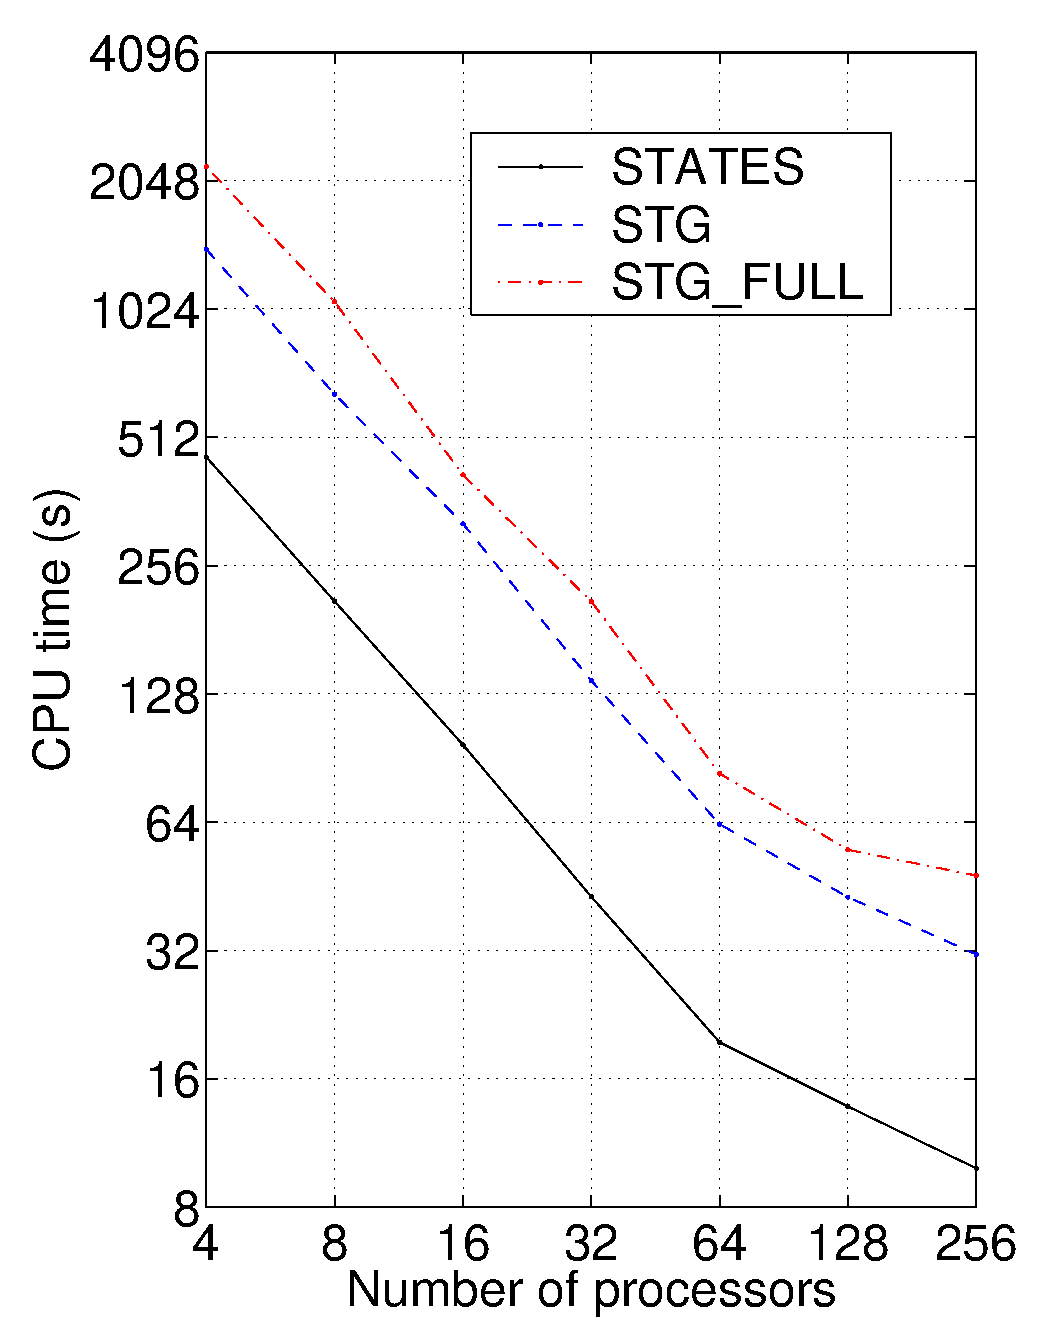
\includegraphics[width=.85\textwidth]{speedup.eps}
  \end{minipage}
  \begin{minipage}[c]{.5\textwidth}
    \centering
    \begin{tabularx}{\textwidth}{cccc}\hline
      $P$ &  STATES  &   STG   & STG\_FULL \\ \hline
      4  &  460.31  &  1414.53  & 2208.14  \\
      8  &  211.20  &   646.59  & 1064.94  \\
     16  &   97.16  &   320.78  &  417.95  \\
     32  &   42.78  &   137.51  &  210.84  \\
     64  &   19.50  &    63.34  &   83.24  \\
     128  &   13.78  &    42.71  &   55.17  \\
     256  &    9.87  &    31.33  &   47.95  \\ \hline
   \end{tabularx}
 \end{minipage}
 \figcaption{Speedup results for the integration of the state equations only
   (solid line and column 'STATES'), staggered sensitivity analysis without
   error control on the sensitivity variables (dashed line and column 'STG'),
   and staggered sensitivity analysis with full error control (dotted line and
   column 'STG\_FULL')}
 \label{f:speedup}
\end{figure}


\section{Availability}\label{s:availability}

The CVODES package has been released under a BSD open source license and is 
freely available at the web site
{\bf www.llnl.gov/CASC/sundials},
or through the DOE ACTS web site at
{\bf acts.nersc.gov/sundials/main.html}.

\section{Conclusions}\label{s:conclusions}

CVODES is the first in a series of new additions to SUNDIALS. The new codes,
IDAS and KINSOLS, together with CVODES, will provide sensitivity analysis
for all the classes of problems addressed by the basic SUNDIALS solvers.
These new capabilities extend the versatility and functionality of the SUNDIALS
solvers in addressing new classes of applications, such as dynamically-constrained
optimization, inversion, and uncertainty quantification.

Like all of SUNDIALS, CVODES is under active development.
An area of particular interest is in the automatic generation of the
sensitivity equations. A parser and code generator for the automatic
generation of derivative approximations using the complex step method
is underway.
Automatic differentiation (AD) tools will be incorporated as they
become available; we are especially interested in adding reverse AD
capabilities to the SUNDIALS adjoint sensitivity solvers.
We are currently investigating alternatives to checkpointing within
the adjoint solver in CVODES: one direction is in using reduced order
models of the forward problem, while another is in storing the
complete decision history on the first forward pass and re-using it on
the second pass.
Finally, to address language interoperability issues and thus
facilitate the use of the SUNDIALS solvers for users of other
programming languages, we plan to generate Babel~\cite{KKPR:01}
wrappers for them.
 


%=======================================================================
% Bibliography
\bibliographystyle{acmtrans}
\bibliography{../biblio}

%=======================================================================
% The article should end by the following lines. 
% The actual dates will be supplied by the Editor-in-Chief.

\begin{received}
Received Month Year;
revised Month Year; accepted Month Year
\end{received}

\end{document}
